\documentclass{pracamgr}
\usepackage{polski}
\usepackage{indentfirst}
\usepackage{parskip}
\usepackage{graphicx}
\usepackage{tabularx}
\usepackage{setspace}
\usepackage{listings}
\usepackage{hyphenat}
\usepackage{mdwlist}
\usepackage{fontspec}
\usepackage{xunicode}
\usepackage{xltxtra}
\usepackage{xeCJK}
\usepackage{url}
\usepackage{booktabs}

\hyphenation{MySQL jQuery}

\setmainfont[Mapping=tex-text,Bold=Charis SIL Bold]{Gentium}
\setsansfont[Mapping=tex-text]{Calibri}
\setmonofont[Scale=0.7]{DejaVu Sans Mono}
\setCJKmainfont[Scale=0.7]{Sazanami Mincho}

\lstset{
	tabsize=4,
	basicstyle=\ttfamily,
	columns=fixed,
	showstringspaces=false,
	extendedchars=true,
	breaklines=true,
	%prebreak = \raisebox{0ex}[0ex][0ex]{\ensuremath{\hookleftarrow}},
	showtabs=false,
	showspaces=false,
	showstringspaces=false,
}

\author{Krzysztof Dudzik}
\nralbumu{248349}
\title{Aplikacja wspomagająca tworzenie i~edycję haseł w~polskim Wikisłowniku}
\tytulang{An application supporting article creation and edition for the Polish Wiktionary}
\kierunek{Informatyka}
\opiekun{dr. hab. Jerzego Tyszkiewicza, prof. UW\\Instytut Informatyki\\}
\date{2011}
\dziedzina{11.3 Informatyka\\}
\klasyfikacja{D. Software\\D.2. Software Engineering\\D.2.10. Design}
\keywords{Wikisłownik, Fundacja Wikimedia, MediaWiki, wiki, edytor, API, JavaScript, jQuery, interfejs użytkownika, społeczność internetowa}

% Tu jest dobre miejsce na Twoje własne makra i~środowiska:
\setkeys{Gin}{width=0.9\textwidth}
\graphicspath{{./screeny/}}
\setlength{\fboxsep}{0pt}
\setlength{\fboxrule}{0.2pt}
\setlength{\parskip}{1.2ex plus 0.5ex minus 0.2ex}
\setlength{\parindent}{5ex}
\frenchspacing
\brokenpenalty=1000
\clubpenalty=1000
\widowpenalty=1000
\renewcommand*{\figurename}{Ilustracja}
\renewcommand*{\listfigurename}{Spis ilustracji}
\newcommand{\spacer}{
	\begin{center}
		\textasteriskcentered
	\end{center}
}
\newcommand{\solidrule}{
	\begin{center}
		\line(1,0){250}
	\end{center}
}
\newenvironment{illustration}[0]{
	\begin{figure}[ht]
	\begin{center}
}{
	\end{center}
	\end{figure}
}
\newenvironment{opis}[0]{
	\begin{basedescript}{\desclabelstyle{\pushlabel}\desclabelwidth{6em}}\setlength{\itemsep}{-2mm}
}{
	\end{basedescript}
}
\let\kod\lstinline


\begin{document}
\maketitle

\begin{abstract}
  Tematem pracy jest aplikacja służąca do ułatwienia pracy autorów haseł w~polskim Wikisłowniku. Jej funkcje mają w~maksymalny możliwy sposób ułatwić tworzenie i~edytowanie haseł osobom bez wiedzy informatycznej i~technicznej, a~także automatyzować możliwie wiele rutynowych czynności wykonywanych przy redagowaniu hasła, jak tworzenie łącz do haseł powiązanych, zautomatyzowane szukanie przykładów użycia, wystąpień w~związkach frazeologicznych, wyrazów bliskoznacznych, innych słów, którą formę gramatyczną mogłoby stanowić hasło~itp. Dodatkowo aplikacja może przejąć część funkcji realizowanych obecnie za~pomocą botów.
\end{abstract}

\tableofcontents

\chapter{Wprowadzenie}
Żyjemy w~czasach, w~których nieustannie zmienia się sposób wyszukiwania informacji przez przeciętnego człowieka. Z~roku na rok coraz mniejszą rolę odgrywają papierowe kompendia takie jak encyklopedie i~słowniki, stopniowo przybierają natomiast na znaczeniu elektroniczne bazy wiedzy -- szczególnie zaś internetowe zbiory danych. Przyczyny tego stanu rzeczy są oczywiste: chodzi przede wszystkim o~wygodę korzystania ze~stron internetowych. Brak możliwości wyszukiwania w~obrębie ogromnych ilości danych powoduje, że encyklopedie i~słowniki w~postaci książek stają się o~wiele mniej atrakcyjne dla kogoś, kto chce zdobyć nowe informacje.

Wszechobecny dostęp do internetu sprawia, że to właśnie w~sieci WWW powstają najbardziej popularne bazy ludzkie wiedzy. Nie ma chyba internautów, którzy nie korzystaliby, rzadziej lub częściej, z~Wikipedii -- internetowej encyklopedii pisanej przez ochotników. Właśnie fakt, że encyklopedia ta współtworzona jest przez amatorów, stanowi o~jej wyjątkowym charakterze, który zostanie w~tej pracy pokrótce opisany. Wikipedia stale utrzymuje się w~pierwszej dziesiątce najczęściej odwiedzanych stron, a~pod wieloma względami jest to dziś najlepsza istniejąca encyklopedia. Przed kilkoma laty głośne było porównanie jej z~prestiżową \emph{Encyclopaedia Britannica} -- okazało się, że różnice w~poziomie merytorycznym są niewielkie.

O~ile przewrót w~kategorii encyklopedii właściwie już się dokonał, nieco inaczej wygląda rywalizacja słowników. Oczywiście wyraźnie widać, że i~tu papierowe edycje są coraz mniej popularne. Różnice uwidaczniają się, gdy przeanalizowana zostanie sytuacja słowników internetowych. Tak zwany siostrzany projekt Wikipedii, Wikisłownik, nie dominuje wśród konkurencji -- zarówno na świecie, jak i~w~Polsce. Przyczyny tego stanu rzeczy są złożone. Autor postanowił skupić się na kilku zagadnieniach, uwidaczniających się w~polskojęzycznej wersji Wikisłownika. W~tym celu konieczne było zbadanie społeczności zaangażowanej w~tworzenie tego projektu. Jego efektem było wykonanie prac programistycznych, których opis stanowi główną część niniejszego opracowania.

W~przypadku wszystkich projektów opartych na silniku programistycznym MediaWiki istotną barierą rozwoju jest sama technologia. Każdy ochotnik ma możliwość uczestniczenia w~rozwoju portalu, wiąże się to jednak z~koniecznością przystosowania się do wymagań stawianych przez oprogramowanie. Edytowanie haseł w~internetowej encyklopedii czy słowniku jest praktycznie niemożliwe dla osoby bez wcześniejszego przygotowania lub znacznej wiedzy techniczno\dywiz{}informatycznej. Oprogramowanie MediaWiki oparte jest bowiem na tzw. wikikodzie (także: wikitekst, wikiskładnia), czyli języku opisu struktury i~wyglądu strony internetowej -- prostszym niż HTML, jednak wciąż nieintuicyjnym dla kogoś, kto nie miał wcześniej do czynienia z~tego typu edytorami. Dlatego wielu potencjalnych współautorów zniechęca się do projektu już przy pierwszej próbie poprawy artykułu.

Aby zmienić tę sytuację, przygotowany został nowy edytor, dostosowany specjalnie do potrzeb polskiego Wikisłownika. Aplikacja pozwala na o~wiele prostsze tworzenie nowych i~zmienianie starych haseł niż poprzednia, standardowa. Dzięki użyciu jej jako domyślnej w~projekcie popularyzacja edytowania Wikisłownika wśród fachowców w~dziedzinach lingwistycznych okaże się łatwiejsze -- zniknie podstawowa bariera, jaką jest konieczność dostosowania się do skomplikowanych technicznych wymagań stawianych przez użyte oprogramowanie. Dodatkowo nowa aplikacja umożliwia zaawansowaną automatyzację tworzenia hasła. Wiele z~czynności zintegrowanych z~nowym edytorem do tej pory wymagało mozolnych poszukiwań w~artykułach Wikisłownika oraz innych projektach. Dzięki użyciu API udostępnianego przez serwisy Fundacji Wikimedia skomplikowane przeszukiwanie tysięcy stron udało się sprowadzić do kilku kliknięć.

W~dalszej części pracy opisany został proces tworzenia tego edytora. Pierwszy rozdział charakteryzuje pokrótce sam Wikisłownik, jak i~pokrewne projekty oraz oprogramowanie w~nich użyte. Następnie opisano społecznościowe aspekty tworzenia tego typu aplikacji ze szczególnym uwzględnieniem koncepcji \emph{wiki}. Ostatni rozdział wyczerpująco przedstawia szczegóły projektowe i~implementacyjne aplikacji.

\chapter{Wikisłownik}
Rozdział ten stanowi charakterystykę Wikisłownika -- sieciowego słownika opartego na oprogramowaniu MediaWiki. Wikisłownik jest jednym z~największych i~najpopularniejszych słowników dostępnych w~polskim internecie. W~kolejnych sekcjach projekt ten został opisany na różnych poziomach szczegółowości. Omówiono zarówno oprogramowanie, na jakim bazuje słownik, jak i~swego rodzaju ,,ekosystem'', w~którym znajduje on swoje miejsce.

\section{Projekty Fundacji Wikimedia}
Podmiotem odpowiedzialnym m.in. za rozwój Wikisłownika jest Wikimedia Foundation Inc.\ (opisywana dalej jako ,,Fundacja'') -- organizacja non\dywiz{}profit mająca siedzibę w~San Francisco w~Stanach Zjednoczonych, istniejąca od 2003 roku. Jak informuje strona internetowa polskiego partnera Fundacji, Stowarzyszenia Wikimedia Polska, \emph{celem fundacji jest sprzyjanie tworzeniu i~rozwojowi projektów o~otwartej treści opartych na technologii WikiWiki oraz dostarczanie społeczności internetowej pełnej zawartości wymienionych projektów za darmo i~bez zamieszczania reklam.} %cite
Doskonale znaną, sztandarową inicjatywą Fundacji jest Wikipedia (\url{http://www.wikipedia.org}) -- największa obecnie encyklopedia internetowa, dostępna w~281 językach (stan z~maja 2011 roku) i~zawierająca ponad 18~milionów haseł, w~tym ponad 3,6~miliona w~największej, angielskojęzycznej\footnote{Oficjalnie w~projektach Fundacji używane są określenia typu \emph{angielskojęzyczny}, \emph{polskojęzyczny}. Choć w~przypadku wersji polskojęzycznej znakomita większość uczestników projektów pochodzi z~Polski, nie jest to regułą dla innych edycji. W~dalszej części pracy przyjęto uproszczenie polegające na tym, że określenia typu \emph{polska Wikipedia}, \emph{angielski Wikisłownik} traktowane są jako tożsame z~określeniami używającymi sformułowań z~cząstką \emph{-języczny}.} edycji. Mimo częstej krytyki tego przedsięwzięcia faktem jest, że Wikipedia jest miejscem, z~którego miliony osób korzystają, by pozyskać informacje z~najróżniejszych dziedzin. Obecny stan rzeczy możliwy jest dzięki pracy wielkiej liczby wolontariuszy tworzących artykuły bez wynagrodzenia.

\begin{illustration}
	\fbox{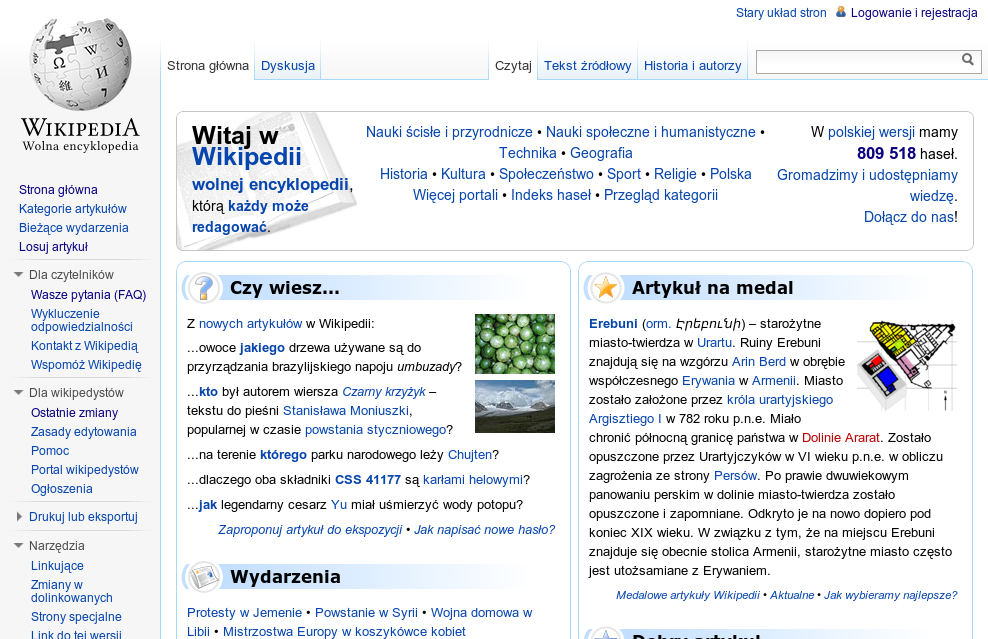
\includegraphics{plwikipedia}}
	\caption{Polska edycja Wikipedii}
\end{illustration}

Wikipedia jest najbardziej znanym, ale nie jedynym projektem pod opieką Fundacji. Pozostałe to tzw.\ ,,projekty siostrzane'', w~szczególny sposób uwzględniane również przy tworzeniu haseł w~encyklopedii. Oto lista wspieranych przez Fundację wielojęzycznych inicjatyw:
\begin{itemize}
	\item Wikisłownik (ang. \emph{Wiktionary}) -- wielojęzyczny słownik internetowy, będący głównym przedmiotem niniejszej pracy,
	\item Wikicytaty (ang. \emph{Wikiquotes}) -- zbiór cytatów autorstwa znanych osób, z~filmów i~książek, przysłów i~porzekadeł,
	\item Wikibooks -- serwis z~,,otwartymi'' (opartymi na wolnej licencji) podręcznikami,
	\item Wikiźródła (ang. \emph{Wikisource}) -- zbiór dokumentów źródłowych w~wersjach oryginalnych i~tłumaczonych, nieograniczonych prawem autorskim,
	\item Wikinews -- otwarty serwis informacyjny,
	\item Wikimedia Commons -- repozytorium mediów (zdjęć, grafik, filmów) dostępnych na wolnej licencji, z~którego korzystają pozostałe projekty Wikimedia,
	\item Wikispecies -- katalog gatunków organizmów żywych,
	\item Wikiversity -- materiały edukacyjne i~naukowe,
	\item Wikimedia Incubator -- metaprojekt umożliwiający tworzenie nowych inicjatyw wspieranych przez Fundację.
	\item Meta\dywiz{}Wiki -- projekt ułatwiający koordynację wszystkich pozostałych.
\end{itemize}
Wszystkie projekty łączy sposób ich powstawania -- możliwość edycji dostępna jest praktycznie dla każdego internauty. Nie dotyczy to co~prawda kilku krajów, w~których projekty Fundacji zablokowane są w~ramach cenzury internetu, jednak ogromna większość osób dysponujących łączem internetowym ma szansę stać się jednymi spośród współautorów haseł.

Drugą cechą wspólną są wolne licencje, na których udostępniana jest zawartość wszystkich serwisów. Po reformie w~czerwcu 2009~roku treść Wikipedii i~projektów siostrzanych dostępna jest nie tylko na licencji GNU FDL (Free Documentation License), ale także na kompatybilnej z~nią CC\dywiz{}BY\dywiz{}SA 3.0 (Creative Commons Attribution\dywiz{}ShareAlike / Uznanie Autorstwa -- Na Tych Samych Warunkach). %cite http://meta.wikimedia.org/wiki/Licensing_update/Result
Oznacza to, że można ją dowolnie wykorzystywać we~własnych dziełach pod warunkiem podania oryginalnych autorów i~zachowania pierwotnej licencji.

\section{Oprogramowanie MediaWiki}
Sama działalność wolontarystyczna redaktorów projektów Wikimedia nie wystarczyłaby do stworzenia serwisów internetowych o~obecnych kształtach. Konieczne jest oczywiście również zapewnienie oprogramowania, które umożliwi płynną współpracę przy tworzeniu haseł. Tym oprogramowaniem jest wolna platforma MediaWiki tworzona zgodnie z~zasadami \emph{open source}. System MediaWiki napisany jest w~języku PHP i~obsługuje kilka popularnych baz danych (w~przypadku projektów Wikimedia jest to MySQL). Dla inicjatyw Wikimedia stanowi szkielet programistyczny od samego ich początku, a~od 2002~roku stale się rozwija. W~czerwcu 2011~roku wersją używaną w~projektach było MediaWiki~1.17.

System MediaWiki używany jest nie tylko w~projektach wspieranych przez Fundację, ale także w~tysiącach innych, mniejszych lub większych, co jest możliwe dzięki wysokiemu stopniowi konfigurowalności i~dużej liczbie dostępnych rozszerzeń. Są to w~dużej mierze serwisy o~podobnym charakterze, umożliwiające swobodną wymianę informacji na dowolny temat. MediaWiki bywa także używane w~firmowych intranetach i~wszędzie tam, gdzie zachodzi potrzeba udostępnienia materiałów do edycji dużej liczbie użytkowników.

\subsection{Edytowanie i~wikitekst}
Strony w~projektach opartych na platformie MediaWiki na~ogół nie mogą być czystym tekstem, pozbawionym formatowania. Przykładowo hasła w~encyklopedii muszą zachowywać określoną strukturę -- występuje więc podział na sekcje, ilustracje, różne rodzaje formatowania (kursywa, wytłuszczenie), przypisy czy powtarzalne fragmenty. Szczególnie istotnym elementem są linki pomiędzy poszczególnymi artykułami, wyróżniające projekty Fundacji na tle ich papierowych, ale też elektronicznych konkurentów. Odnośniki pozwalają błyskawicznie przemieszczać się między hasłami, by w~ten sposób uzyskiwać kolejne informacje wspomagające przyswajanie wiedzy.

Linki i~formatowanie na stronach internetowych tworzone są za pomocą elementów języka HTML lub XHTML. O~ile języki te są proste w~obsłudze dla specjalisty informatyka, to laik nie jest w~stanie tworzyć za ich pomocą stron bez uprzedniego dłuższego przygotowania. Aby umożliwić bezproblemową edycję stron internetowych osobom bez wykształcenia informatycznego, programiści MediaWiki zaprojektowali tzw.\ wikitekst -- uproszczony język opisu stron, pozwalający na realizację wymienionych elementów. Porównanie niektórych z~nich znajduje się w~tabeli \ref{tab:html-wiki}.

\begin{table}[h]
\begin{center}
\footnotesize{
	\begin{tabularx}{\textwidth}{ lXX }
		\toprule & Wikitekst & XHTML \\
		\toprule Kursywa & \texttt{''Tekst''} & \texttt{<em>Tekst</em>} \\
		\midrule Wytłuszczenie & \texttt{'''Tekst'''} & \texttt{<strong>Tekst</strong>} \\
		\midrule Nagłówek & \texttt{== Nagłówek ==} & \texttt{<h2>Nagłówek</h2>} \\
		 & \texttt{=== Nagłówek ===} & \texttt{<h3>Nagłówek</h3>} \\
		\midrule Odnośnik wewnętrzny & \texttt{[[Strona]]} & \texttt{<a href="/wiki/Strona">Strona</a>} \\
		 & \texttt{[[Strona|strony]]} & \texttt{<a href="/wiki/Strona">strony</a>} \\
		\midrule Odnośnik zewnętrzny & \texttt{[http://www.google.com Google]}
		 & \texttt{<a href="http://www.google.com">\newline Google</a>} \\
		\midrule Obraz & \texttt{[[Plik:Przykład.png|thumb|Podpis]]} & \texttt{<img src="$\ldots$ /Przykład.png"/><br/>\newline <div class="caption">Podpis</div>} \\
		\midrule Podział na akapity & \texttt{Pierwszy akapit \newline \newline Drugi akapit}
		 & \texttt{<p>Pierwszy akapit</p>\newline <p>Drugi akapit</p>} \\
		\midrule Lista nienumerowana & \texttt{* Element\newline * Element\newline * Element}
		 & \texttt{<ul>\newline <li>Element</li>\newline <li>Element</li>\newline <li>Element</li>\newline </ul>}\\
		\midrule Lista numerowana & \texttt{\# Element\newline \# Element\newline \# Element}
		 & \texttt{<ol>\newline <li>Element</li>\newline <li>Element</li>\newline <li>Element</li>\newline </ol>}\\
		\bottomrule
	\end{tabularx}
}
\caption{Porównanie HTML i wikitekstu}
\label{tab:html-wiki}
\end{center}
\end{table}

Łatwo można zauważyć, że używanie wikitekstu jest o~wiele prostsze niż nauka XHTML\dywiz{}a. Jeśli zachodzi potrzeba zaawansowanego formatowania, możliwe jest także użycie znaczników XHTML. W~przypadku standardowego formatowania jest to jednak niewskazane ze względu na dobro niedoświadczonych edytorów.

Bardzo istotnym elementem wikitekstu są szablony -- predefiniowane fragmenty kodu z~opcjonalnymi parametrami. Szablony można uznać za odpowiednik procedur/funkcji w~językach programowania. W~projektach opartych na MediaWiki szablony pełnią przede wszystkim dwie główne funkcje:
\begin{itemize}
	\item upraszczają kod -- pozwalają np.\ na zastąpienie skomplikowanego kodu XHTML (a~także jeszcze bardziej złożonych funkcji parsera MediaWiki) krótkim wywołaniem szablonu,
	\item standaryzują strony -- często wykorzystywane fragmenty wywoływane są zawsze w~dokładnie ten sam sposób.
\end{itemize}
We~wszystkich większych projektach Fundacji szablony są bardzo często wykorzystywane. Przy tym stanowią duże ułatwienie dla technicznie zaawansowanych autorów, którzy wspomagają się przy tworzeniu haseł dodatkowymi technologiami. Na używaniu szablonów korzystają przede wszystkim boty, czyli programy dokonujące edycji samodzielnie po uprzednim przygotowaniu lub pod stałą opieką programisty. W~większości projektów przyjęte jest, że każdy bot ma własne konto użytkownika, nie używa natomiast konta swojego ,,właściciela''. Dzięki botom możliwe jest np.\ masowe tworzenie haseł w~Wikipedii na ściśle określony temat, jeśli istnieje dobre źródło w~formie czytelnej dla komputera (takich jak opisy asteroid czy wszystkich miejscowości lub jednostek administracyjnych w~danym kraju). Innym ich zastosowaniem jest automatycznie uzupełnianie tzw.\ interwiki -- czyli odnośników pomiędzy poszczególnymi wersjami językowymi tego samego hasła.

Szablony mogą być wykorzystywane w~prosty sposób nawet przez początkujących użytkowników -- aby wywołać szablon, wystarczy wpisać jego nazwę
 pomiędzy podwójnymi nawiasami klamrowymi (\kod@{{Nazwa szablonu}}@ lub \kod@{{Nazwa szablonu|parametr=abc}}@). W~polskim Wikisłowniku szablony pełnią szczególną rolę -- i~to m.in.\ dzięki ich szerokiemu zastosowaniu w~projekcie zrodził się pomysł na niniejszą pracę. Szczegóły tego zagadnienia zostaną przedstawione w~sekcji~\ref{sec:plwikt}.

\section{Wiktionary -- Wikisłownik}
\begin{illustration}
	\fbox{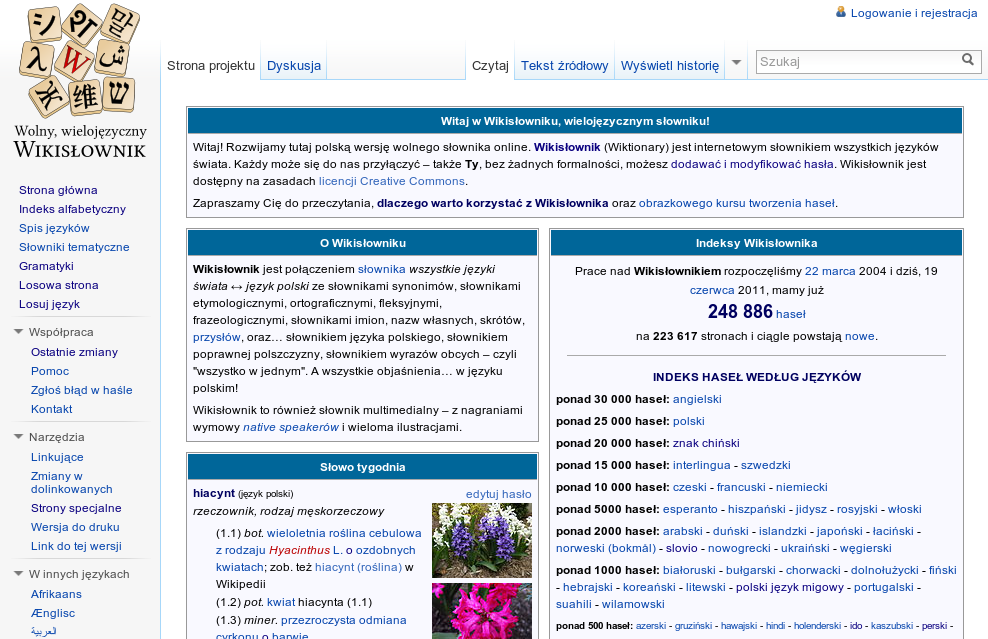
\includegraphics{plwikt}}
	\caption{Polska edycja Wikisłownika}
\end{illustration}
Jednym z~największych projektów siostrzanych Wikipedii jest Wikisłownik, w~wersji angielskiej (i~wielu innych) noszący nazwę \emph{Wiktionary} (\url{http://www.wiktionary.org}). Ten słownik internetowy nie rozwinął się jeszcze tak prężnie jak encyklopedia, zwłaszcza jeśli chodzi o~polską edycję. Jest dziś jednak jednym z~największych słowników w~sieci, a~w~pewnych zastosowaniach stanowi najlepszy wybór. Dużą zaletą Wikisłownika jest jego wielojęzyczność -- w~tym samym serwisie znaleźć można hasła w~ponad~250~językach. W~przypadku niektórych z~nich jest to praktycznie jedyny słownik internetowy lub nawet jedyny dostępny słownik w~ogóle. Przykładem może być polski Wikisłownik, który zawiera prawdopodobnie jedyny polski słownik języka hawajskiego czy największe słowniki języków suahili i~jidysz. %cite http://pl.wiktionary.org/wiki/Wikis%C5%82ownik:Dlaczego_Wikis%C5%82ownik

Wspomniane zostało zastosowanie szablonów do standaryzacji kodu źródłowego i~struktury haseł. Trzeba jednak zaznaczyć, że dotyczy to wyłącznie haseł w~obrębie jednej wersji językowej Wikisłownika, są one bowiem niezależne od siebie i~od Fundacji. Wspólne dla wszystkich edycji jest jedynie oprogramowanie MediaWiki i~umiejscowienie na serwerach Fundacji pod adresem \kod|xxx.wiktionary.org|, gdzie zamiast \kod|xxx| wstawiany jest dwu- lub trzyliterowy skrót ISO języka (np. \url{pl.wiktionary.org} = język polski, \url{de.wiktionary.org} = język niemiecki, \url{sq.wiktionary.org} = język albański, \url{csb.wiktionary.org} = język kaszubski). Wszystkie kwestie organizacyjne w~obrębie wersji językowej ustalane są w~ramach dyskusji i~głosowań przez internetową społeczność. Głosowania służą także wyborowi administratorów projektu, czyli użytkowników mających dodatkowe uprawnienia, spośród których najważniejsze to usuwanie i~zabezpieczanie haseł oraz blokowanie użytkowników działających na szkodę projektu. W~lipcu 2011~roku w~angielskim Wikisłowniku działało aktywnie 76~administratorów, %cite http://en.wiktionary.org/wiki/Wiktionary:Administrators
zaś w~polskim -- 14. %cite http://pl.wiktionary.org/wiki/Wikis%C5%82ownik:Administratorzy
Dla porównania Wikipedia w~języku angielskim ma 1541~administratorów (niekoniecznie aktywnych), wersja polska natomiast 163. %cite http://meta.wikimedia.org/wiki/Administrators_of_various_Wikipedias

Podobnie jak w~przypadku Wikipedii, hasła w~poszczególnych wersjach językowych Wikisłownika są łączone poprzez odnośniki interwiki, znajdujące się na dole lewego menu w~większości haseł. W~stosunku do encyklopedii występuje znacząca różnica w~sposobie funkcjonowania tych linków. Wikipedia poprzez interwiki łączy artykuły na ten sam temat, często różniące się tytułem (polski artykuł \emph{Kot domowy} odsyła do angielskiego \emph{Cat} czy niemieckiego \emph{Hauskatze}). W~Wikisłowniku mechanizm interwiki łączy zaś strony o~tym samym tytule, niezależnie od ich zawartości. Polskie hasło \emph{kot} zawiera więc łącza do haseł o~tytule \emph{kot} w~innych językach, które mogą, ale nie muszą zawierać m.in.\ objaśnienia polskiego znaczenia tego słowa. Z~tego względu łatwo jest odnaleźć brakujące informacje o~wybranym słowie w~danym języku, jeśli skorzysta się z~kilku edycji językowych Wikisłownika. Natomiast tłumaczenia tytułu hasła na inne języki znajdują się bezpośrednio w~treści artykułu, w~miejscu przeznaczonym dla takich informacji.

Choć poszczególne wersje Wikisłownika różnią się między sobą, wspólna jest struktura hasła na najogólniejszym poziomie. Każde hasło jest podzielone na sekcje nagłówkami 2.~stopnia (patrz tabela \ref{tab:html-wiki}), podobnie jak w~innych projektach Fundacji. W~przypadku słownika sposób podziału artykułu został jasno sprecyzowany i~jest wspólny dla wszystkich edycji. W~każdej z~sekcji objaśniono znaczenie tytułowego hasła w~innym języku. Przykładowo hasło \emph{nie} w~większości wersji językowych ma sekcje objaśniające znaczenie m.in.\ w~języku polskim oraz języku niemieckim (\emph{nigdy}). Właśnie ta ogólna cecha struktury haseł pozwala na częściową automatyzację niektórych często wykonywanych w~trakcie edycji czynności.

Aplikacja opisana w~niniejszej pracy przeznaczona jest dla polskiej edycji Wikisłownika. Konieczne jest zatem scharakteryzowanie specyfiki tego projektu (patrz sekcja \ref{sec:plwikt}). Ze~względu na odmienność poszczególnych wersji językowych prawdopodobnie w~innych nie będzie można wykorzystać wykorzystać aplikacji. Z~pewnością może ona być dla nich jednak bardzo przydatna -- duża część funkcji przez nią realizowanych może być używana niezależnie od specyfiki danej wersji, a~budowa aplikacji pozwoli na ich wyodrębnienie.

\section{Polska edycja Wikisłownika}
\label{sec:plwikt}
Wikisłownik w~języku polskim powstał 22 marca 2004 r. %http://pl.wiktionary.org/wiki/Wikis%C5%82ownik:Strona_g%C5%82%C3%B3wna
i~jest dziś jedną z~najlepiej rozwiniętych edycji. Jeśli chodzi o~liczbę haseł, polska wersja zawiera ich ponad 230~000 i~znajduje się na 8.~miejscu (pierwsze trzy miejsca zajmują z~dużą przewagą edycje angielska, francuska i~chińska). Warto zwrócić jednak uwagę, że liczba artykułów nie musi odzwierciedlać ogólnego poziomu rozwoju danej edycji, a~przynajmniej w~o~wiele mniejszym stopniu niż w~Wikipedii. Automatyczne importowanie haseł słownikowych z~innych źródeł jest prostsze niż w~przypadku wpisów do~encyklopedii, a~hasła takie oczywiście nie wyróżniają się pozytywnie pod względem jakości. Wydaje się, że lepszym wskaźnikiem rozwoju są np.\ liczby aktywnych użytkowników lub administratorów. Tutaj polski Wikisłownik okazuje się wielokrotnie lepszy niż edycje litewska czy malajska, górujące nad nim pod względem liczby haseł.
%http://meta.wikimedia.org/wiki/Wiktionary#List_of_Wiktionaries

W~kolejnej podsekcji opisana została dokładnie struktura haseł w~polskim Wikisłowniku. Społeczność tego projektu scharakteryzowano natomiast w~sekcji \ref{sec:plsoc}.

\subsection{Struktura hasła}
Jak wspomniano, wspólny dla wszystkich wersji językowych Wikisłownika jest podział na sekcje, odpowiadające poszczególnym językom. Polska edycja Wikisłownika jest bardzo dobrze ustrukturyzowana w~dalszym zakresie, co niekoniecznie jest regułą dla pozostałych edycji. Wynikiem tego jest jednolity wygląd hasła, który otrzymuje czytelnik, oraz jednolity kod widziany przez redaktora. Przykładowy artykuł z~jedną sekcją językową znajduje się na ilustracji \ref{fig:plhaslo}.

\begin{illustration}
	\fbox{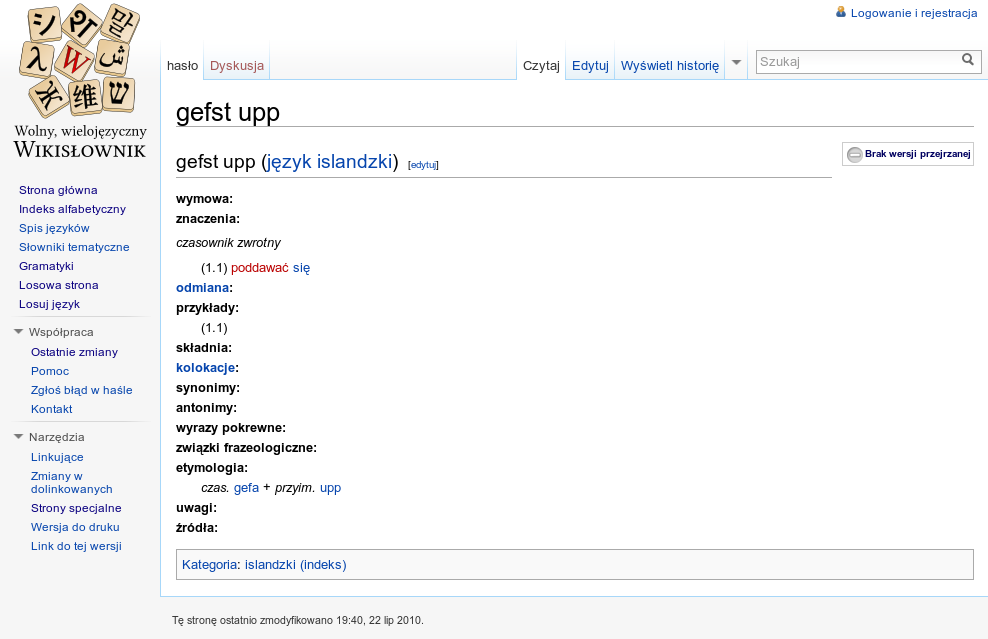
\includegraphics{plwikt-art}}
	\caption{Hasło \emph{gefst upp} w~polskim Wikisłowniku (\protect\url{http://pl.wiktionary.org/wiki/gefst_upp})}
	\label{fig:plhaslo}
\end{illustration}

Na zrzucie ekranu widoczny jest układ sekcji typowy dla polskiego projektu. Z~małymi wyjątkami sekcje danego języka wyglądają tak samo we~wszystkich hasłach. To oznacza, że także w~innych opisanych wyrazach języka islandzkiego znaleźć można elementy: wymowa, znaczenia, odmiana, przykłady, składnia, kolokacje, synonimy, antonimy, wyrazy pokrewne, związki frazeologiczne, etymologia, uwagi, źródła. W~rzeczywistości jest to układ typowy dla znakomitej większości występujących w~Wikisłowniku języków. Odstępstwa od tego szkieletu hasła są niewielkie i~zostaną przedstawione poniżej.

Ilustracja \ref{fig:plhaslo-edit} przedstawia wygląd przykładowej strony po przejściu do trybu edycji, dostępnego dla każdego użytkownika (bez konieczności logowania). Widok ten prezentuje źródłowy wikikod hasła, dodatkowo edytor ma kilka ikon ułatwiających wstawianie często używanych elementów. W~kodzie tym widoczne są szablony definiujące tytuły poszczególnych elementów sekcji (nazywanych dalej \emph{podsekcjami}). Podział na sekcje i~podsekcje jest dość prosty do wykonania za pomocą programu komputerowego i~już sama ta procedura pozwala na znaczne zwiększenie przejrzystości w~nowym edytorze, opisanym w~rozdziale \ref{chap:impl}.

\begin{illustration}
	\fbox{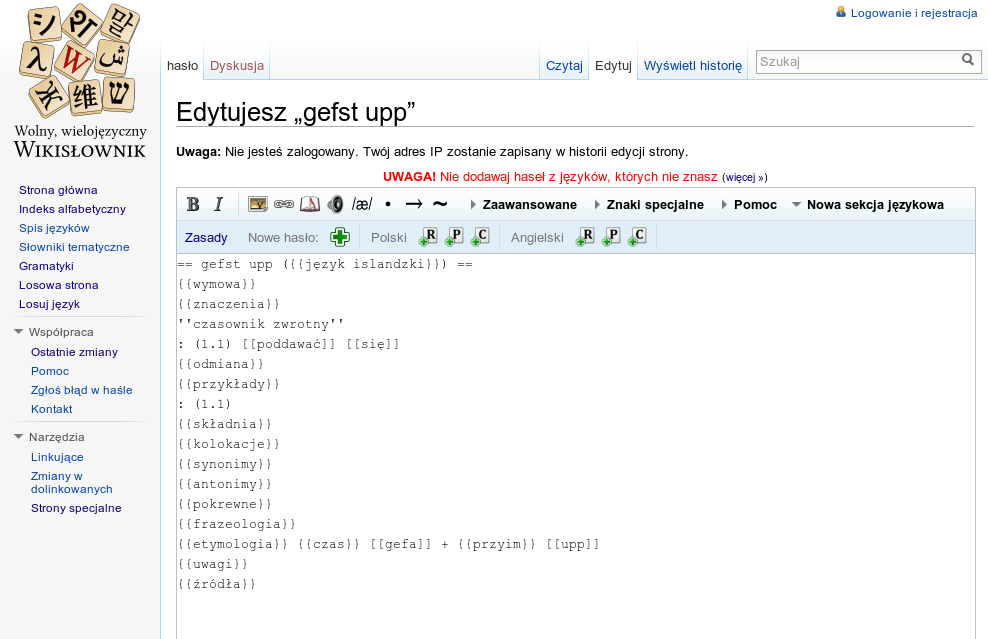
\includegraphics{plwikt-edit}}
	\caption{Edycja hasła \emph{gefst upp} w~polskim Wikisłowniku (\protect\url{http://pl.wiktionary.org/w/index.php?title=gefst_upp&action=edit})}
	\label{fig:plhaslo-edit}
\end{illustration}

Każda z~podsekcji w~hasłach ma ściśle określoną funkcję, dzięki której polski Wikisłownik jest jednolity. Poniżej zostały omówione wszystkie podsekcje występujące w~artykułach, w~jedynej przyjętej jako poprawną kolejności. Duża ich część pojawia się jedynie w~niektórych językach, dlatego choć lista podsekcji jest dość długa, to każde hasło będzie miało ich o~wiele mniej. Szablony podsekcji zebrane są na stronie \url{http://pl.wiktionary.org/wiki/Kategoria:Szablony_szablonów_haseł}.
\subsubsection{Podsekcje występujące w~hasłach polskiego Wikisłownika}

\begin{opis}
	\item[Szablon] \verb|{{zapis hieroglificzny}}|
	\item[Zawartość] Zapis hieroglificzny słowa w~języku staroegipskim, pokazany za~pomocą grafik PNG z~repozytorium Wikimedia Commons. Oznaczenie \kod|(1.1)| odnosi się do numeracji w~sekcji \emph{znaczenia}.
	\item[Języki] tylko staroegipski\footnote{Rubryka \emph{Języki} precyzuje, w~których sekcjach językowych występuje dana podsekcja. Oprócz zwykłych sekcji, odpowiadających danemu językowi, istnieją także nietypowe: \emph{użycie słowa obcego w~języku polskim} i~\emph{znak chiński}}.
	\item[Przykład]
		\begin{verbatim}
			{{zapis hieroglificzny}}
			: (1.1) [[Plik:Egyptian-Pr-cnḫ.PNG]];
			[[Plik:Egyptian-Pr-cnḫ2.PNG]];
			[[Plik:Egyptian-Pr-cnḫ3.PNG]]
		\end{verbatim}
\end{opis}
\spacer
\begin{opis}
	\item[Szablon] \verb|{{ortografie}}|
	\item[Zawartość] Inne sposoby zapisu tytułu hasła. Zazwyczaj chodzi o~alternatywną pisownię w~języku, do zapisu którego używane są dwa alfabety (np.\ serbski). Do prezentacji pisowni mogą być używane szablony wyświetlające dodatkowe informacje.
	\item[Języki] azerski, białoruski, dżuhuri, gagauski, krymskotatarski, ladino, serbski, slovio, tatarski, turkmeński, ujgurski
	\item[Przykład]
		\begin{verbatim}
			{{ortografie}} Мацедониа
		\end{verbatim}
\end{opis}
\spacer
\begin{opis}
	\item[Szablon] \verb|{{transliteracja}}|
	\item[Zawartość] Transliteracja słowa zapisanego w~obcym alfabecie na alfabet łaciński. W~przeciwieństwie do transkrypcji transliteracja może być wykonywana automatycznie -- każda litera alfabetu obcego konwertowana jest na jeden lub więcej znaków w~alfabecie łacińskim. Obecnie często używany jest szablon \kod|{{translit}}|, który umożliwia automatyczną konwersję za pomocą JavaScriptu niektórych alfabetów podczas odczytywania strony.
	\item[Języki] abazyński, abchaski, adygejski, akadyjski, amharski, arabski, aramejski, assamski, awarski, baszkirski, beludżi, bengali, birmański, bośniacki, bułgarski, chakaski, czeczeński, czuwaski, dzongkha, erzja, gocki, gruziński, gudźarati, gyyz, hebrajski, hindi, inguski, inuktitut, jidysz, kannada, kaszmirski, kazachski, khmerski, kirgiski, komi, komi\dywiz{}jaźwiński, kri, kurdyjski, laotański, lezgiński, macedoński, malajalam, malediwski, marathi, maryjski, mongolski, nepalski, newarski, nowogrecki, orija, ormiański, osetyjski, paszto, pendżabski, perski, romski, rosyjski, sanskryt, sindhi, sorani, staro\dywiz{}cerkiewno\dywiz{}słowiański, starogrecki, staroormiański, sumeryjski, syngaleski, tabasarański, tadżycki, tajski, tamazight, tamilski, telugu, tybetański, ukraiński, urdu, zarfatit
	\item[Przykład]
		\begin{verbatim}
			{{transliteracja}} Moskva
		\end{verbatim}
\end{opis}
\spacer
\begin{opis}
	\item[Szablon] \verb|{{transkrypcja}}|
	\item[Zawartość] Transkrypcja słowa zapisanego w~obcym alfabecie na język polski, czyli przedstawienie go w~formie dającej informacje o~rzeczywistej wymowie
	\item[Języki] standardowo tylko staroegipski, podsekcja ta może być jednak dodawana w~wielu innych językach (przykład w~jidysz)
	\item[Przykład]
		\begin{verbatim}
			{{transkrypcja}}
			: (1.1-3) {{YIVO|{{lp}} khaver {{lm}} khaveyrim}}; polska: {{lp}}
			chawer {{lm}} chawejrim
			: (1.4) {{YIVO|{{lp}} khover {{lm}} khovers}}; polska: {{lp}}
			chower; {{lm}} chowers
		\end{verbatim}
\end{opis}
\spacer %http://pl.wiktionary.org/wiki/Kategoria:Szablony_szablon%C3%B3w_hase%C5%82
\begin{opis}
	\item[Szablon] \verb|{{czytania}}|
	\item[Zawartość] Wyjaśnienie możliwego wymawiania znaków kanji używanych w~języku japońskim. Występują dwa sposoby czytania: on'yomi i~kun'yomi. Do ich prezentacji używane są szablony \kod|{{on}}| i~\kod|{{kun}}|.
	\item[Języki] tylko japoński
	\item[Przykład]
		\begin{verbatim}
			{{czytania}} {{on}} ビ (bi); {{kun}} はな (hana)
		\end{verbatim}
\end{opis}
\spacer
\begin{opis}
	\item[Szablon] \verb|{{klucz}}|
	\item[Zawartość] Elementy, według których układane są słowniki języka chińskiego.
	\item[Języki] tylko znak chiński
	\item[Przykład]
		\begin{verbatim}
			{{klucz}} 157 足 + 6
		\end{verbatim}
\end{opis}
\spacer
\begin{opis}
	\item[Szablon] \verb|{{kreski}}|
	\item[Zawartość] Liczba kresek użytych do napisania danego znaku. Informacja służy m.in.\ do ułatwienia odnajdywania znaków w~papierowych słownikach.
	\item[Języki] znak chiński, koreański
	\item[Przykład]
		\begin{verbatim}
			{{kreski}} 13
		\end{verbatim}
\end{opis}
\spacer
\begin{opis}
	\item[Szablon] \verb|{{warianty}}|
	\item[Zawartość] Szablon powiększający znak chiński i~ewentualnie jego warianty. Szablon ten jest używany inaczej niż większość: nie odpowiada jedynie za wyświetlenie nagłówka, a~zawartość sekcji wstawiana jest jako parametr. Najczęściej w~parametrze pojawia się szablon \kod|{{zch-w}}|, odpowiadający za prezentację znaku.
	\item[Języki] tylko znak chiński
	\item[Przykład]
		\begin{verbatim}
			{{warianty|{{zch-w}}}}
		\end{verbatim}
\end{opis}
\spacer
\begin{opis}
	\item[Szablon] \verb|{{kolejność}}|
	\item[Zawartość] Kolejność stawiania kresek w~znaku chińskim, ilustrowana za pomocą grafiki dostępnej w~projekcie Wikimedia Commons. W~tej podsekcji używane są szablony \kod|{{zch-komiks}}|, \kod|{{zch-cienie}}| i~\kod|{{zch-animacja}}|, które ładują automatycznie grafiki o~nazwie odpowiadającej hasłu, jeśli te istnieją.
	\item[Języki] tylko znak chiński
	\item[Przykład]
		\begin{verbatim}
		{{kolejność}}
		{{zch-komiks}}
		\end{verbatim}
\end{opis}
\spacer
\begin{opis}
	\item[Szablon] \verb|{{wymowa}}|
	\item[Zawartość] Jedna z~kluczowych podsekcji we~wszystkich językach. Podawane są w~niej informacje na temat wymowy danego hasła, zarówno za pomocą alfabetów fonetycznych (jak np.\ IPA oraz alfabet słowiański), jak i~nagrań dźwiękowych umieszczonych w~Wikimedia Commons. Do opisywania wymowy stosowane są szablony \kod|{{IPA}}|, \kod|{{IPA2}}|, \kod|{{IPA3}}|, \kod|{{IPA4}}|. Wymowa słów polskich dodawana jest automatycznie przez bota uruchomionego przez jednego z~administratorów Wikisłownika. Bot ten jest skomplikowanym programem napisanym w~Javie, generującym wymowę na podstawie publikacji Ostaszewskiej i~Tambora. %cite
	Pliki dźwiękowe dodawane są szablonem \kod|{{audio}}|.
	\item[Języki] wszystkie poza znakiem chińskim i~użyciem międzynarodowym
	\item[Przykład]
		\begin{verbatim}
		{{wymowa}} {{audio|Pl-samochód.ogg}}, {{IPA3|sãˈmɔxut}}, {{AS3|sãm'''o'''χut}},
		{{objaśnienie wymowy|WYG|NAZAL}}
		\end{verbatim}
\end{opis}
\spacer
\begin{opis}
	\item[Szablon] \verb|{{znaczenia}}|
	\item[Zawartość] Jedyna podsekcja obowiązkowa, w~której podawane jest znaczenie hasła. Zawartość podsekcji dzielona jest najpierw na części mowy, potem na poszczególne znaczenia, które zostają ponumerowane zgodnie z~obowiązującym schematem. W~hasłach polskich podawane jest dłuższe znaczenie, w~innych językach tłumaczenie na polski. Znaczenia te są linkami do objaśnień form podstawowych poszczególnych słów -- linkowanie to stanowi dość duże utrudnienie przy tworzeniu hasła.
	\item[Języki] wszystkie
	\item[Przykłady] Hasło angielskie:
		\begin{verbatim}
		{{znaczenia}}
		''rzeczownik''
		: (1.1) [[zamówienie]]
		: (1.2) [[rozkaz]]
		: (1.3) [[porządek]]
		: (1.4) {{syst}} [[rząd]]
		: (1.5) {{mat}} [[rząd]]
		''czasownik''
		: (2.1) [[zamawiać]]
		: (2.2) [[rozkazywać]]
		\end{verbatim}
		Hasło polskie:
		\begin{verbatim}
		{{znaczenia}}
		''rzeczownik, rodzaj męski''
		: (1.1) [[budynek]] [[warowny]]; {{wikipedia|zamek (architektura)}}
		: (1.2) [[mechanizm]] [[zamykać|zamykający]] [[drzwi]], [[szuflada|szuflady]];
		{{wikipedia|zamek (urządzenie)}}
		: (1.3) [[zapięcie]] [[garderoba|garderoby]], {{zob|[[zamek błyskawiczny]]}}.
		: (1.4) [[element]] [[składowy]] [[broń|broni]] [[palny|palnej]];
		{{wikipedia|zamek (broń)}}
		: (1.5) {{sport}} [[w]] [[hokej]]u: [[zamykać|zamknięcie]] [[przeciwnik]]a [[w]]
		[[tercja|tercji]], [[gdy]] [[drużyna]] [[atakować|atakująca]]
		[[rozgrywać|rozgrywa]] [[krążek]] [[w]] [[tercja|tercji]] [[przeciwnik]]a [[nie]]
		[[pozwalać|pozwalając]] [[on|mu]] [[wyjść]] [[poza]] [[niebieski|niebieską]]
		[[linia|linię]]
		\end{verbatim}
\end{opis}
\spacer
\begin{opis}
	\item[Szablon] \verb|{{determinatywy}}|
	\item[Zawartość] Znak określający, o~jaką klasę znaczeniową wyrazów chodzi w~danym haśle. Wyświetlana jest grafika z~Wikimedia Commons.
	\item[Języki] tylko staroegipski
	\item[Przykład]
		\begin{verbatim}
			{{determinatywy}}
			: (1.1) [[Plik:Egyptian-nb ʿnḫ-determinative.PNG]]
		\end{verbatim}
\end{opis}
\spacer
\begin{opis}
	\item[Szablon] \verb|{{odmiana}}|
	\item[Zawartość] Odmiana wyrazu, prezentowana na różne sposoby. Występują np.\ szablony, które generują odmianę na podstawie formy podstawowej hasła. Niekiedy podawana jest jedynie deklinacja lub koniugacja (z~odnośnikiem do tabel ją przedstawiających), gdzie indziej cała odmiana.
	\item[Języki] wszystkie poza znakiem chińskim
	\item[Przykład]
		\begin{verbatim}
			{{odmiana}}
			: (1.1-2) читать {{ter}} {{lp}} читаю, читаешь, читает; {{lm}} читаем, читаете,
			читают; {{przesz}} {{lp}} читал / читала / читало; {{lm}} читали; {{rozk}} {{lp}}
			читай; {{ims}} читающий; читаемый; читая
		\end{verbatim}
\end{opis}
\spacer
\begin{opis}
	\item[Szablon] \verb|{{przykłady}}|
	\item[Zawartość] Przykłady użycia danego słowa w~zdaniu. W~przypadku języków innych niż polski tłumaczenie przykładu podane jest po znaku →. Podobnie jak znaczenia, przykłady są linkowane.
	\item[Języki] wszystkie poza znakiem chińskim
	\item[Przykład]
		\begin{verbatim}
			{{przykłady}}
			: (2.1) ''[[Michael]] '''locks''' [[his]] [[house]] [[every]] [[day]]. '' →
			[[Michał]] [[codziennie]] '''[[zamykać|zamyka]]''' [[swój]] [[dom]] (na klucz).
		\end{verbatim}
\end{opis}
\spacer
\begin{opis}
	\item[Szablon] \verb|{{składnia}}|
	\item[Zawartość] Podsekcja zawiera informacje o~używaniu słowa w~połączeniu z~przyimkami czy przypadkami.
	\item[Języki] wszystkie poza znakiem chińskim
	\item[Przykład]
		\begin{verbatim}
			{{składnia}}
			: (1.2) jechać +{{N}}; jechać [[do]] +{{D}}, jechać [[na]] +{{B}}
		\end{verbatim}
\end{opis}
\spacer
\begin{opis}
	\item[Szablon] \verb|{{kolokacje}}|
	\item[Zawartość] Kolokacje to często używane zestawienia słów, w~których (w~przeciwieństwie do związków frazeologicznych) znaczenie całości wynika ze znaczenia poszczególnych wyrazów.
	\item[Języki] wszystkie poza znakiem chińskim
	\item[Przykład]
		\begin{verbatim}
			{{kolokacje}} [[mieć]] / [[budzić]] / [[odbierać]] nadzieję • [[promyk]]
			nadziei • [[ziścić]] nadzieje • [[karmić]] [[się]] nadzieją
		\end{verbatim}
\end{opis}
\spacer
\begin{opis}
	\item[Szablon] \verb|{{synonimy}}|
	\item[Zawartość] Wyrazy bliskoznaczne, synonimy.
	\item[Języki] wszystkie poza znakiem chińskim
	\item[Przykład]
		\begin{verbatim}
			{{synonimy}}
			: (1.1) [[ufność]], [[wiara]], [[zawierzenie]], [[pociecha]]
		\end{verbatim}
\end{opis}
\spacer
\begin{opis}
	\item[Szablon] \verb|{{antonimy}}|
	\item[Zawartość] Wyrazy przeciwstawne, antonimy
	\item[Języki] wszystkie poza znakiem chińskim
	\item[Przykład]
		\begin{verbatim}
			{{antonimy}}
			: (1.1) [[rezygnacja]], [[zwątpienie]], [[beznadzieja]]
		\end{verbatim}
\end{opis}
\spacer
\begin{opis}
	\item[Szablon] \verb|{{złożenia}}|
	\item[Zawartość] W~językach japońskim i~koreańskim podsekcja ta podaje słowa, które powstają jako złożenie danego hasła z~innym. Użyty w~przykładzie szablon \kod|{{furi}}| pomaga dobrze wyświetlić furiganę -- japońskie pismo.
	\item[Języki] koreański i~japoński
	\item[Przykład]
		\begin{verbatim}
			{{złożenia}} {{furi|五日|いつか}}, {{furi|五月|ごがつ}},
			{{furi|五輪|ごりん}}, {{furi|五輪大会|ごりんたいかい}}
		\end{verbatim}
\end{opis}
\spacer
\begin{opis}
	\item[Szablon] \verb|{{pokrewne}}|
	\item[Zawartość] Wyrazy pokrewne do danego wyrazu podstawowego. W~przypadku większej grupy wyrazów wspólnej dla wielu haseł może wystąpić odsyłacz do wyrazu podstawowego, np. w~haśle \emph{kocur}: \kod@{{zob|[[kot]]}}@.
	\item[Języki] wszystkie poza znakiem chińskim
	\item[Przykład]
		\begin{verbatim}
			{{pokrewne}}
			: (1.1) {{rzecz}} [[picklock]], [[locksmith]], [[locknut]]
			: (1.2) {{rzecz}} [[dreadlock]]
			: (1.3) {{rzecz}} [[airlock]], [[lockage]]
			: (2.1) {{przym}} [[lockable]]; {{rzecz}} [[locker]]
		\end{verbatim}
\end{opis}
\spacer
\begin{opis}
	\item[Szablon] \verb|{{pochodne}}|
	\item[Zawartość] Odpowiednik podsekcji \emph{pokrewne} dla morfemów w~esperanto, stanowiących osobne hasła.
	\item[Języki] esperanto
	\item[Przykład]
		\begin{verbatim}
			{{pochodne}} {{rzecz}} [[zebro]], [[zebrino]], [[zebrido]]
		\end{verbatim}
\end{opis}
\spacer
\begin{opis}
	\item[Szablon] \verb|{{frazeologia}}|
	\item[Zawartość] Podsekcja zawiera związki frazeologiczne, które prezentowane są podobnie jak kolokacje. Różnica między kolokacjami a~związkami frazeologicznymi polega na tym, że w~przypadku tych drugich znaczenie związku nie wynika bezpośrednio ze znaczeń poszczególnych wyrazów.
	\item[Języki] wszystkie poza znakiem chińskim
	\item[Przykład]
		\begin{verbatim}
			{{frazeologia}}
			: [[psi urok]] • [[tu leży pies pogrzebany]] • {{wulg}} [[pies kogoś jebał]] •
			[[pies ogrodnika]] • {{pot}} [[pies na baby]] • [[pogoda pod psem]] • [[psu na
			budę]] • [[pieskie życie]] • [[psia wachta]] • [[psia koja]] • [[pies
			Pawłowa]] • [[nie dla psa kiełbasa]] • [[pies łańcuchowy Darwina]] • [[na psa
			urok]] • [[ni pies, ni wydra]] • [[schodzić na psy]] • [[łgać jak pies]] •
			[[delikatny jak francuski piesek]] • [[francuski piesek]] • [[pies z nim
			tańcował]] • [[psi żywot]] • [[psie figle]] • [[psi obowiązek]] • [[całować
			psa w nos]] • [[wyć jak pies do księżyca]] • [[żyć jak pies z kotem]] •
			[[wieszać na kimś psy]] • [[lubić kogoś jak psy dziada w ciasnej ulicy]] •
			[[robić coś psim swędem]] • [[wyglądać jak zbity pies]] • [[być wyszczekanym
			jak pies]] • [[psia kość]] • [[kupować za psie pieniądze]] • [[wyszczekać coś
			jak pies]] • [[odszczekać coś jak pies]] • [[wierny jak pies]] • [[pies ci
			mordę lizał]]
			: zobacz też: [[Aneks:Przysłowia polskie - zwierzęta#pies|przysłowia o psie]]
		\end{verbatim}
\end{opis}
\spacer
\begin{opis}
	\item[Szablon] \verb|{{etymologia}}|
	\item[Zawartość] Pochodzenie wyrazu, zapisywane za pomocą szablonów \kod|{{etym}}| i~\kod|{{etymn}}|.
	\item[Języki] wszystkie
	\item[Przykład]
		\begin{verbatim}
			{{etymologia}}
			: {{etym|prasłowiański|*ne}} < {{etym|praindoeuropejski|*ne}} 'nie'
			: {{por}} {{etymn|czeski|ne}}, {{etymn|rosyjski|не}}, {{etymn|litewski|ne}},
			{{etymn|łaciński|ne}}
		\end{verbatim}
\end{opis}
\spacer
\begin{opis}
	\item[Szablon] \verb|{{kody}}|
	\item[Zawartość] Informacje na temat wprowadzania znaków chińskich za pomocą klawiatury w~różnych metodach oraz kodowania Unicode. Podobnie jak w~przypadku podsekcji \emph{warianty}, i~tutaj szablon przyjmuje parametry pozwalające na zestandaryzowane wyświetlanie.
	\item[Języki] tylko znak chiński
	\item[Przykład]
		\begin{verbatim}
			{{kody |cjz=田金 |cjl=WC |cr=6021<sub>0</sub> |u=56db}}
		\end{verbatim}
\end{opis}
\spacer
\begin{opis}
	\item[Szablon] \verb|{{hanja}}|
	\item[Zawartość] W~tej podsekcji podawana jest pisownia danego słowa koreańskiego w~piśmie hanja (hancha), czyli pisownia zapożyczona z~języka chińskiego. Częściej w~koreańskim używany jest alfabet hangul.
	\item[Języki] tylko koreański
	\item[Przykład]
		\begin{verbatim}
			{{hanja}} [[憲法]]
		\end{verbatim}
\end{opis}
\spacer
\begin{opis}
	\item[Szablon] \verb|{{słowniki}}|
	\item[Zawartość] Informacja na temat występowania danego znaku chińskiego w~słownikach KangXi, Dai Kanwa Jiten, Dae Jaweon i~Hanyu Da Zidian.
	\item[Języki] tylko znak chiński
	\item[Przykład]
		\begin{verbatim}
			{{słowniki|kx=1163.080|dkj=35533|dj=1628.020|hdz=63974.090}}
		\end{verbatim}
\end{opis}
\spacer
\begin{opis}
	\item[Szablon] \verb|{{uwagi}}|
	\item[Zawartość] Dodatkowe informacje, np.\ częste błędy, odpowiedzi na typowe wątpliwości.
	\item[Języki] wszystkie
	\item[Przykład]
		\begin{verbatim}
			{{uwagi}}
			: (1.1) forma ''tylni'' dla przymiotnika rodzaju męskiego w liczbie pojedynczej
			jest błędna, może odnosić się ona jedynie do liczby mnogiej<ref>{{PoradniaPWN|id=
			9687|hasło=tylny czy tylni?}}</ref>
		\end{verbatim}
\end{opis}
\spacer
\begin{opis}
	\item[Szablon] \verb|{{tłumaczenia}}|
	\item[Zawartość] Podsekcja ta pełni funkcję słownika z~języka polskiego na inne. Podawane są odnośniki do wyrazów będących tłumaczeniami danego słowa polskiego.
	\item[Języki] tylko polski
	\item[Przykład]
		\begin{verbatim}
			{{tłumaczenia}}
			* angielski: (1.1) [[date]], [[appointment]]
			* arabski: (1.1) [[تعيين]]
			* francuski: (1.1) [[rendez-vous]]
			* rosyjski: (1.1) [[свидание]], {{pot}} [[свиданка]]
			* szwedzki: (1.1) [[träff]] {{w}}
		\end{verbatim}
\end{opis}
\spacer
\begin{opis}
	\item[Szablon] \verb|{{źródła}}|
	\item[Zawartość] Źródła dla informacji podanych w~haśle. Zazwyczaj sekcja ta składa się ze znacznika \kod|<references/>|, który powoduje wyświetlenie w~tym miejscu przypisów wstawionych w~poprzedzającej zawartości strony znaczników \kod|<ref>...</ref>|.
	\item[Języki] wszystkie
	\item[Przykład]
		\begin{verbatim}
			{{źródła}}
			<references/>
		\end{verbatim}
\end{opis}
\spacer

\subsubsection{Wady dotychczasowych rozwiązań}
W~obecnym systemie edycji w~Wikisłowniku przedstawiona wyżej regularna struktura nie jest wykorzystywana w~wystarczającym stopniu. W~dużej mierze wiąże się to z~pierwotnym założeniem, jakim jest oparcie projektu na silniku MediaWiki. Każde hasło przechowywane jest w~bazie danych jako jeden ciąg znaków, a~ich struktura jest wymuszona dopiero przez społeczność -- brakuje jakichkolwiek mechanizmów, które pomagałyby w~utrzymywaniu haseł zgodnie ze standardem.

Baza Wikisłownika nie zachowuje zatem nawet pierwszej postaci normalnej %cite
-- hasła nie są wszak danymi atomowymi. To duża wada projektu takiego jak słownik internetowy, w~którym dane powinny być prezentowane możliwie jednolicie. Postaci normalne pozwalają też na łatwiejszą modyfikację i obróbkę danych. Niestety niemożliwa jest zmiana silnika MediaWiki, dlatego należy dbać o~standaryzację artykułów za pomocą innych środków.

Ilustracja \ref{fig:plnew} pokazuje to i~owo.

\begin{illustration}
	\fbox{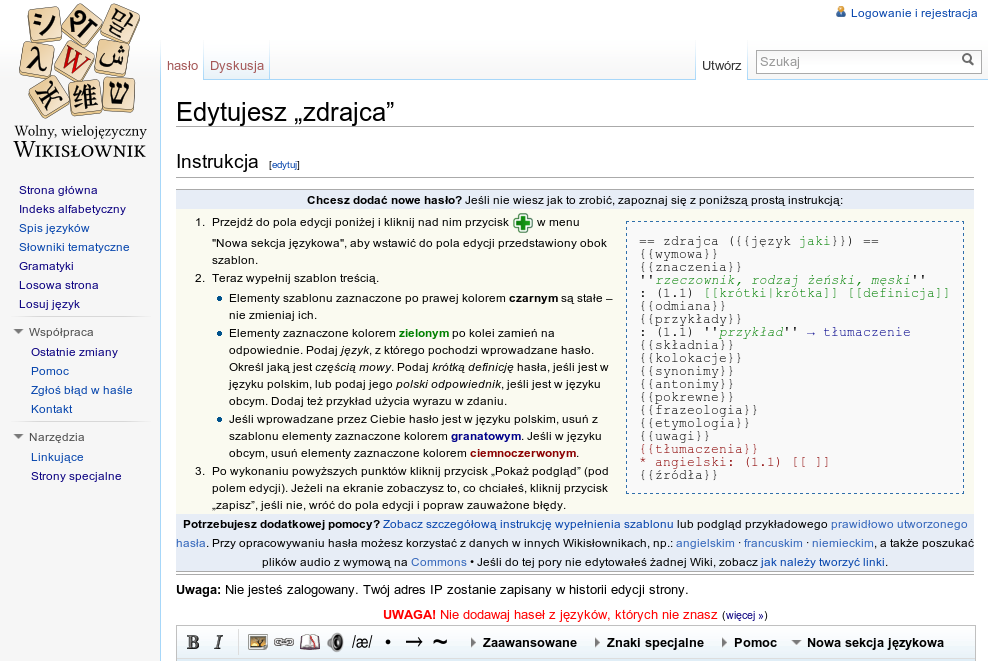
\includegraphics{plwikt-edit-non}}
	\caption{Próba stworzenia nowego hasła w~polskim Wikisłowniku}
	\label{fig:plnew}
\end{illustration}

\chapter{Aspekty społecznościowe}
\section{Koncepcja \emph{wiki}}
\section{Społeczność polskiej edycji Wikisłownika}
\label{sec:plsoc}

\section{Specyfika tworzenia aplikacji dla wikispołeczności}

\chapter{Opis implementacji}
\label{chap:impl}
\section{Wprowadzenie}
\section{Formularz edycyjny}
\section{Automatyzacja edycji hasła}
\section{Wdrożenie}

\chapter{Podsumowanie}


\appendix

\cleardoublepage
\addcontentsline{toc}{chapter}{Bibliografia}
\printbibliography[title={Bibliografia}]
\newpage
\addcontentsline{toc}{chapter}{Spis ilustracji}
\listoffigures
\addcontentsline{toc}{chapter}{Spis tabel}
\listoftables

\end{document}
